\section{The Peer-to-Peer Network Architecture}
In a Peer-to-Peer (P2P) network every node acts as both client and
server. Every node contributes with its resources, including both
storage space and processing power. The execution of the system is
determined by a decentralized algorithm, which every node in the P2P
network must follow. No node has global knowledge of the entire network,
and no node acts as a single point of failure. This ensures a high
degree of scalability in terms of number of queries or amount of data
being processed, as every node is able to act as a server. Also, the P2P
network architecture is highly resilient to churn, as each node
independently needs to handle joins and leaves gracefully. This type of
self-organization is one of the main characteristics of the P2P network
architecture.

\section{Overlays}
The logical connections between participants in a P2P
system lies on top of the physical connections on the network. This
means that a one-hop connection between two peers might in reality
consist of several hops between separate machines at the physical layer.
The higher level connections between peers forms what is called an
\emph{overlay}, as they form a logical network at a higher abstraction
level that facilitates routing, search and key-value storage. Typically,
overlays are separated into two different types of networks: structured
and unstructured. The former organizes nodes into structures such as
trees or rings, while the latter aims to form an overlay which resembles
a random graph. Structural overlays introduce overhead in terms of
structural maintenance but are able to provide higher guarantees of
correct message delivery than random overlays.

\section{The Publish-Subscribe Communication Paradigm}
Publish-Subscribe is a fully asynchronous, loosely coupled,
highly scalable, event-based messaging pattern. There are three main
system components in the pub/sub interaction scheme: the publishers, the
subscribers and the event service. The publishers publish events, and
the subscribers subscribe for events, while the event service handles
managing both subscriptions and publications, as well as routing events
to the subscribers. The basic architecture of a typical pub/sub system
is outlined in Figure~\ref{fig:pubsubarch}.

\begin{figure}
\centering
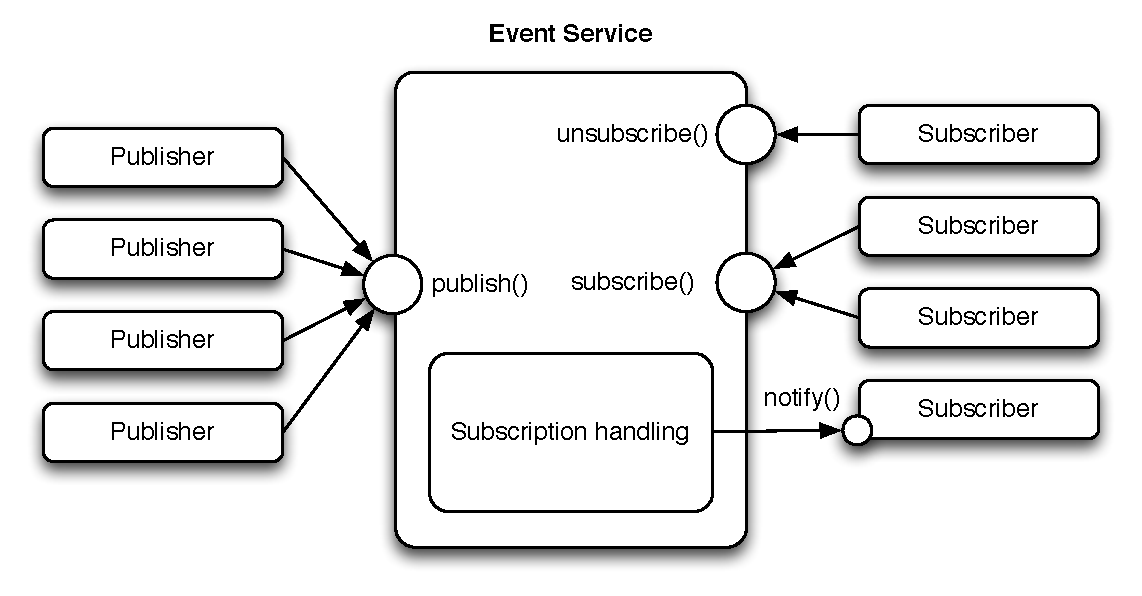
\includegraphics[width=\textwidth]{figures/pubsubarch}
\caption{The basic architecture of a pub/sub system.}
\label{fig:pubsubarch}
\end{figure}

The event service functions as an intermediary between publishers and
subscribers. It provides a level of indirection, as well as an service
interface. Publishers are able to generate new events through the
\texttt{publish} service call. It is now the responsibility of the event
service to determine which subscribers are interested in receiving this
event, and how to route the event to them. The subscribers register
their interest through a \texttt{subscribe} service call. The event
service will then store each subscribers interest in order to
disseminate events correctly. The publishers are then able to cancel
their subscriptions through a \texttt{unsubscribe} service call. No
information is forwarded from subscribers to publishers or from
publishers to subscribers.

The pub/sub paradigm provides a higher degree of decoupling than other
traditional approaches. In general there are three types of decoupling
pub/sub system provides us with:

\begin{description}
  \item[Space decoupling] The publishers and subscribers does not need to
    know about each other.
  \item[Time decoupling] Events are delivered regardless of whether or
    not publishers and subscribers are online at the same time.
  \item[Synchronization decoupling] Neither publishers nor subscribers
    are blocked when attempting to perform their operations.
\end{description}

While many other approaches can provide the first two forms of
decoupling, the main advantage of pub/sub is its fully asynchronous nature.
Approaches such as tuple spaces or message queues cannot completely
provide this synchronous decoupling, as messages are retrieved in a
synchronous manner. This property is key to the suitability for pub/sub
in large distributed system.~\cite{Eugster:2003}

\subsection{Message Filtering in Pub/Sub}

The subscription semantics of the pub/sub paradigm plays an important
role in the performance and flexibility of the system as event messages
are routed and managed based on topic or content. There are three
distinct types of subscription schemes:

\begin{description}
  \item[Topic-based] Events are split into topics, usually represented by
      a string.
  \item[Type-based] Filters events based on the structure of the data.
      Provides type safety at compile time.
  \item[Content-based] Events are filtered based on a global
      list of universal event attributes.
\end{description}

Content-based provides better expressiveness in terms of filtering out
the relevant events. However, this comes at the cost of higher overhead
with regards to handling subscriptions. The complex filtering algorithms
limit the scalability of such systems with regards to the number of
subscriptions. Type based is similar to content-based in the sense that
the public members of the types together form a description of the
content of the event. Although this ties the implementation of the
pub/sub system closer to the programming language, it still suffers from
the same drawbacks as content-based.

Topic-based offer less expressiveness than the other two subscription
schemes, but better performance if the set of possible event properties
is limited. Also, topic-based is more suited for dissemination and
multicasting, as topics can be thought of as groups, where subscribing
to topic T can be equivalent to joining the group for that topic. This
is a common approach taken by several proposed pub/sub
systems\cite{needs citation}.

Traditionally, reliable multicasting of data through deterministic
dissemination has been the common approach. However, more recent
implementations investigate the potentials of probabilistic protocols,
which are more suited to the nature of decentralized systems and P2P.
These protocols do not guarantee full reliability, but provides a high
quantifiable \emph{probability} that events are delivered to all
subscribers.

\section{The Gephi Open Graph Viz Platform}

\begin{figure}
    \centering
    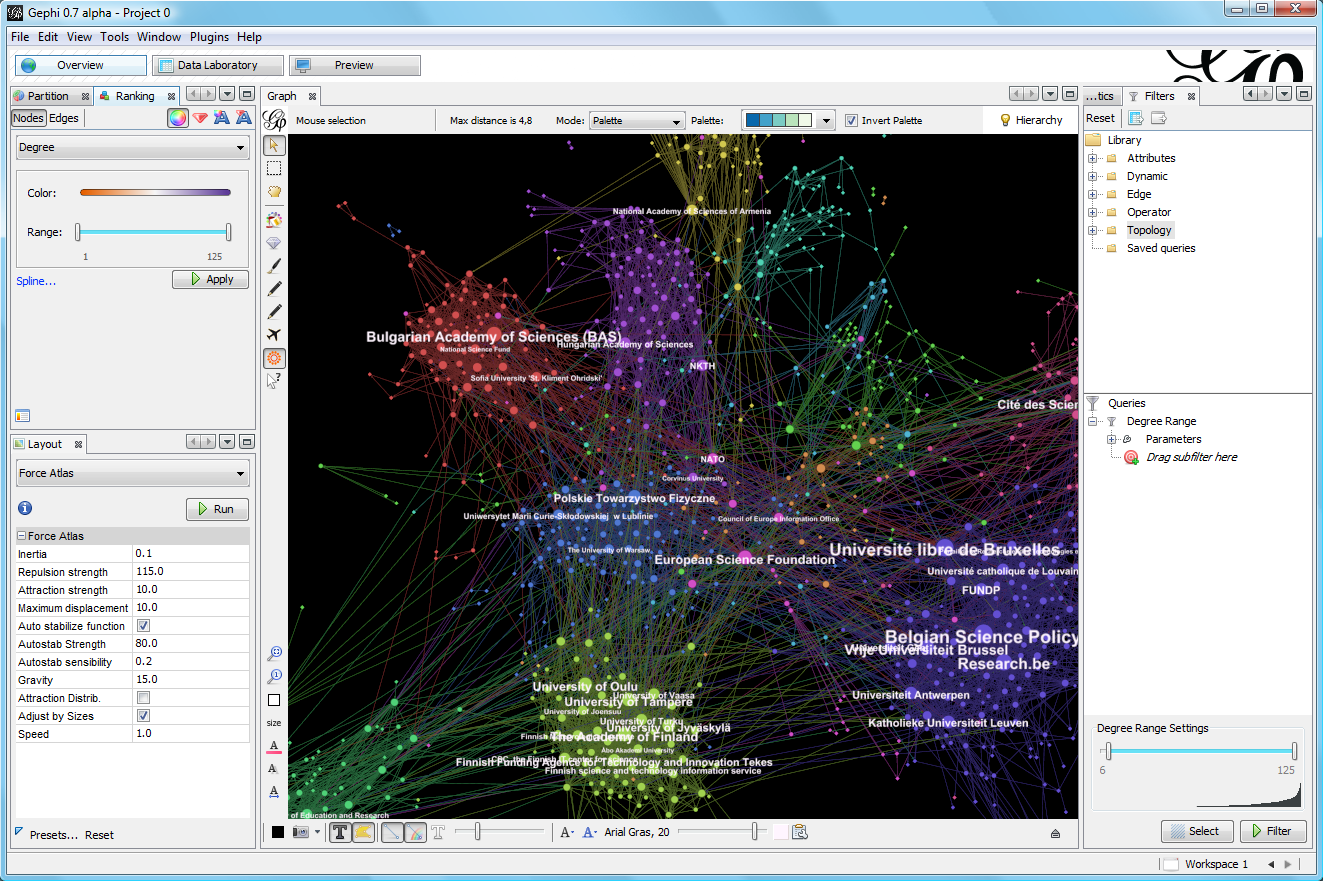
\includegraphics[width=\textwidth]{img/gephi1}
    \caption{The Gephi Tool supports
        visualization of graphs through coloring and sizing the visual
        graph
        representation. It also enables adding labels to nodes and
        edges. In
        this screenshot, Gephi is used to detect and visualize
    communities.}
\label{img:gephi1}
\end{figure}

Gephi~\cite{ICWSM09154} is an open source tool for exploring and
visualizing all kinds of networks, including dynamic and hierarchical
graphs. Described by the authors as ``photoshop for graphs'', Gephi
enables the user to interact with the graph structure, as well as
manipulate the colors and sizes of the visual graph representation in
order to display graph properties in an intuitive way. Gephi aims to
help researchers and data analysts in discovering patterns and revealing
hidden properties of the graph in question, as well as easily
discovering errors in the dataset. Gephi also provides a set of
statistical tools for measuring common metrics for Social Network
Analysis~(SNA) such as centrality, as well as metrics useful for general
graph topology analysis such as degree, path length and clustering
coefficient. Gephi is also useful in the emerging field of Dynamic
Network Analysis~(DNA)  as it supports temporal graphs, giving the user
the ability to filter the graph model according to a defined time
interval. It also support playback of the graph evolution, as well as
visualizing changes to graph data over time through size, color and text
labels which can be applied to both nodes and edges.

Gephi provides a rich GUI-experience where the user may interact with the
graph representation, apply layout algorithms, filter the graph
representation, execute metrics, apply color and size based on graph
properties and animate the graph evolving over time through the timeline
component. The Gephi software architecture is highly modular and
supports extensions via plugins, some of which are available in a
official plugin marketplace found at~\cite{gephimarketplace}. New
metrics, filters or database support may be implemented through such
plugins by developers and published to the marketplace free of charge.

Gephi provides many tools and components which are useful in the context
of researching and analysing pub/sub overlays.

\subsection{Useful functionality in Gephi}

\begin{description}

\item[Node and Edge pencil tools] \hfill \\

    These two tools enable the user to create nodes and edges by
    clicking in the graph view. Edges can be undirected or directed,
    where direction is indicated with an arrow. These two tools combined
    enables building a graph by hand.

    Building such graphs can be useful in order to reason, analyse or
    learn network algorithms, such as event dissemination algorithms. In
    this case, the user can start with a single node which can act as
    the event source, and build the topology as the event disseminates,
    carefully following the particular algorithm in question when doing
    so. The user can also add attributes to the nodes and edges either
    through the node query tool or in the Data Laboratory component
    which also aids in visualising and understanding properties,
    drawbacks and advantages of such algorithms.

\item[Node Query Tool] \hfill \\

    With the node query tool the user is able to click on a node on the
    graph model, and a panel which will display a panel with information
    regarding the properties and attributes of this node. Properties include
    data describing the visual properties of the node such as size, position
    and color. Attributes include the Id and Label and Time Interval
    attributes and any additional user defined attributes. In our case, such
    user defined attributes would include Topics, Subscription Size and
    Gossips Sent/Received.

    Both the properties and attributes of the node are editable through this
    panel view. The user can select a property to change the visual
    representation of the node, or the attributes to change their value. The
    Time Interval attribute is interesting to edit in particular as it
    represents the points in time in which a node exists in the graph model.
    On example scenario is editing the Time Interval attribute for a certain
    nodes in order to see how it affects a particular metric as well as the
    overlay topology.

\item[Shortest Path Tool] \hfill \\

    With the Shortest Path Tool selected, the user may click on two nodes on
    the graph model, and if there is a shortest path between them, this path
    will be highlighted with a color. It might be useful to reason about the
    relationship between key nodes in the graph, or to compare shortest path
    between several pairs of nodes. (more use cases?)

\item[Heat Map Tool] \hfill \\

    The heat map tool enables the user to click on a node in the graph model
    and color its neighborhood based on the edge weight distance between
    them. More specifically, it sets the node color intensity lower for more
    distant nodes and stronger for nodes that are closer. Edge weight is a
    standard edge attribute that are by default set to 1. This means that in
    the default case, the visualization will represent the hop count
    distance from the particular node selected by the user. However, the
    edge weight can be edited by the user in order to represent other
    properties of a system. As an example, imagine setting the edge weight
    to represent network latency between two nodes. In this case, a
    neighboring node which is adjacent to the selected node would have a
    lower color intensity if the latency between them is higher than another
    neighboring node which is further away in terms of hop count.

\item[Timeline Component] \hfill \\

    The timeline component introduces an animation scheme for dynamic
    graphs. The user may choose playback parameters such as time
    interval size, step size and playback speed. The time interval will
    filter out a subgraph defined by the upper and lower bound of the
    interval. The evolution of the dynamic graph will then be animated
    by moving these bounds by the distance defined by the step
    parameter. The delay between each step is decided by the playback
    speed.

    The timeline enables the user to visually inspect the change in
    graph topology over time, as well as visualize and inspect node and
    edge attributes of the graph through both color, size and text
    labels which is able to change dynamically as part of the graph
    model animation. The timeline also enables jumping to a specific
    point in time and investigating the corresponding subgraph and its
    properties by changing the upper and lower bound of the Time
    Interval.

\item[Statistics Component] \hfill \\

    The metric component enables graph topology analysis by executing
    metrics on the graph. There are two types of metric algorithms in Gephi:
    static and dynamic. Static metrics are only able to execute on graph
    model representing a single point in time, while dynamic will traverse
    the time line by executing the metric iteratively across a set of time
    intervals. When executing a dynamic metric, the user is able to choose
    window size and time step. The window size is a time interval which will
    be moved by the step size defined by the user. Metrics are divided
    into \emph{static} and \emph{dynamic} metrics, where the former
    calculates a single value based on the currently defined time
    window, while the latter calculates a time series of values. When
    executing a dynamic metric, the user must define the time window
    size, and tick. The have the same functionality as step parameter
    when using the \emph{Timeline Component}. When the metric executes,
    the time window will iterate through the entire time range of the
    simulation, calculating a static metric at each step. When finished,
    a time series is plotted and displayed for the user.

    The Statistics component include several metrics which are relevant
    to pub/sub overlays. Useful static metrics include, but are not
    limited to:

    \begin{itemize}
        \item{Degree (In/Out/Avg./Max/Min/Distr.)}
        \item{Avg. Cluster Coefficient}
        \item{Centrality (Beetweeness/Closeness/Eccentricity)}
        \item{Average Path length}
        \item{Radius}
        \item{Network Diameter}
        \item{Number of Shortest Paths}
    \end{itemize}

    Of these, only degree and the clustering coefficient metrics have dynamic
    versions, where both calculates the average value over time. The
    average for dynamic metrics are calculated by dividing the sum of
    all node attribute values with the total number of nodes in both
    cases.

    %TODO: describe exactly what sort of averages/data are calculated by
    each metric

\item[Ranking Component] \hfill \\

    The ranking component is a key feature of Gephi which enables
    visualization based on node or edge attributes in form of color
    and size. When coloring nodes or edges, the ranking component
    will apply a gradient over the range of attribute values. The
    ranking component also include a Result list, where the user may
    sort nodes based on the specified attribute value, which is
    useful for quickly finding the nodes with maximum value and
    minimum value, which might help in identifying bottlenecks in
    the system or potential load balancing issues.

    The Ranking component also includes an Auto Apply feature, which
    supports vizualising attributes dynamically while playing back the
    graph via the Timeline Component.

\item[Layout Component] \hfill \\

    The Layout component enables the user to execute algorithms that
    calculates the position of the nodes. The user is able to adjust the
    parameters of these algorithms in order to manipulate the visual
    layout. The different algorithms emphasize different aspects of the
    topology. One example is the Force Atlas layout algortihm which
    simulates the effect of gravity on the nodes where linked nodes
    attract each other, and non-linked nodes are pushed apart. This
    particular algorithm is useful for visually detect clusters and
    communities. Another useful algorithm is the Circular Layout
    algorithm, where nodes are positioned in a circle ordered on a
    specific attributes selectable by the user. This is useful in order
    to visualize node rankings on particular attributes.

\item[Filter Component] \hfill \\

    Filter may be applied to the graph in order to strip away nodes or
    edges on the basis of their attributes which also includes any
    calculated metrics. Filters may strip away based on a value range if
    the attribute type is a number, or a regex match if the attribute is
    a string. Filters can be combined through special operator filters
    representing set operations such as union and intersect.

    Filters are an essential mechanism in order to analyze subgraphs.
    One use example is the case of calculating topic diameters in pub/sub systems,
    where a subgraph can be filtered on a topic attribute. This
    allows executing the diameter metric on the resulting subgraph
    on the selected topic.

\item[Data Laboratory Component] \hfill \\

    The Data laboratory component enables the user to work with the node
    and edge attributes of the graph. This component provides the user
    with separate table views of node and edge attributes. Each row in
    these table represent a node or edge, and columns may be added or
    removed by the user. The Data Laboratory also provides functionality
    for manipulating columns such as merging two columns or creating new
    columns based on data from the existing columns. Attribute data
    in columns that are static (i.e.\ has no lower or upper time
    interval bound associated with them) can be converted to dynamic
    through this component. Also, resizing or coloring all edges or
    nodes is possible through the laboratory by selecting all rows
    and right-clicking.

    The laboratory also enables the user to export the data to file
    for further statistical analysis.
\end{description}

We consider tools such as Gephi to be a valuable addition to the field
of P2P protocol research. Visual Exploration of a dynamic network graph
is a useful approach to evaluating these protocols, as some properties
of the system are more easily spotted visually. For example, during our
implementation work, it was trivial to visually confirm that some edges
were missing from the graph, leading to the discovery of a critical bug
in the implementation code which would otherwise be difficult to spot.
It is also worth to note that the different actors involved in the Gephi
project has formed a legal entity in the form of The Gephi
Consortium~\cite{gephi-consortium} in order to assure future development
of this tool. This provides us with a certain degree of assurance that
this project is something well worth investing in, as the risk of it
being discontinued seems unlikely at this point in time.

\section{The Gephi Toolkit}

In addition to the GUI-client, the authors of Gephi also provide an API
through the Gephi Toolkit project. The toolkit packages essential
modules from the GUI-client into a standard Java library which can
be used by any stand-alone Java project by including it as a dependency.
We take advantage of this toolkit in our implementation work, where it
is mainly used to handle and store reports collected from PeerNet
simulations.

\section{The GEXF File format}

The GEXF (Graph Exchange XML Format) file format~\cite{gexf} is an
effort by the Gephi Consortium to define a standard language describing
complex network structures. Being developed by the same group of people,
the Gephi Tool is naturally fully compatible with this format, and is
able to both import and export GEXF files. This is also the case with
the Gephi Toolkit, as the module for handling such imports and exports
are included in this toolkit as well.

The GEXF file format is able to describe a graph through its nodes and
edges, as well as any data and dynamics associated with the graph. More
specifically, the file format is able to describe node, edges and their
associated attributes. Listing~\ref{lst:gexf-basic} provides an example
of a minimal static GEXF file, describing nodes, edges and attributes of
a graph.

\begin{figure}
\lstinputlisting[language=XML, label=lst:gexf-basic, frame=single]{listings/basic.gexf}
\caption{A GEXF description of a minimal static graph}
\end{figure}

\subsection{Dynamics}

One of the major advantages of this file format is its support for
dynamic functionalities.  Both nodes, edges and attributes may have a
defined time interval where they exist. These lifetime intervals are
described as ``spells'' if applied to nodes and edges, and as ``start''
and ``end'' XML-attributes if applied to node or edge attributes. The
GEXF file in Listing~\ref{lst:gexf-dynamics} shows an example of a
dynamic graph where spells are used in order to determine the lifetime
of the nodes. The start and end times are by default encoded as
floating point values, however, dates are also supported, as seen in this example.

The support for dynamic graphs makes this file format an interesting
option for storing simulation data, and in our implementation work we
use this format extensively as part of our research effort.

\begin{figure}
\lstinputlisting[language=XML, caption={}, label=lst:gexf-dynamics,
frame=single] {listings/dynamics.gexf}
\caption{Example of  dynamic GEXF file using spells}
\end{figure}


\section{Pub/Sub Protocols}
We use two different pub/sub protocols for creating visualizations and
evaluating performance. Both protocols provide a message dissemination
scheme, where nodes are organized in a structured overlay. We briefly
describe the relevant details regarding each protocol, as we later will
provide visualizations of both the structure of these systems as well as
their dissemination scheme.

\subsection{PolderCast}
PolderCast~\cite{Setty:2012} is a topic-based P2P pub/sub system which
organizes nodes in a ring structure. The system architecture of
PolderCast is highly modular, and includes three separate layers of
overlay-based protocols. The CYCLON peer sampling service~\cite{Voulgaris:2005} is used
in order to maintain connectivity across the whole set of subscribers,
as well as providing the rings layer with uniform random links. The
Vicinity module consist of the generic VICINITY protocol, which let
nodes find neighbors based on a \emph{proximity function}. This enables
the ring layer to determine its ring neighbors based on the unique id of
nodes. All the protocol modules rely on gossiping for structural
maintenance. This means that at periodic intervals, a node $p$ will pair up with a
neighbor $q$ and exchange information regarding neighbors and
subscriptions.

\begin{figure*}
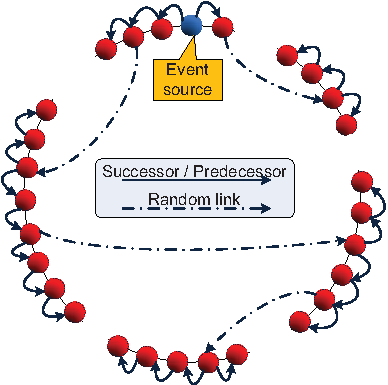
\includegraphics{img/hybrid_dissemination.pdf}
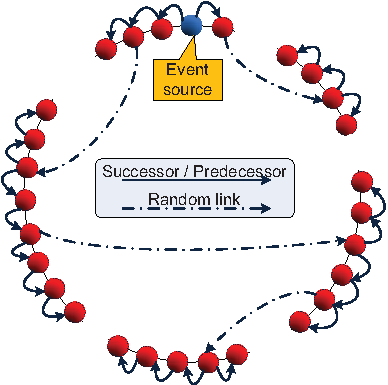
\includegraphics{img/hybrid_dissemination.pdf}
\caption{PolderCast utilizes a hybrid dissemination scheme when
    publishing messages}
\end{figure*}

PolderCast include a hybrid publication scheme using both
ring neighbors and random links in order to boost
dissemination, as well as increase resistance to ring
partitions and churn. The dissemination algorithm is based
on a configurable fanout $f$, and can be summarized in the
following steps for each node:

\begin{enumerate}
    \item If the message has already been received, discard it.
    \item If the message was received from a ring neighbor, forward it
        to the other ring neighbor, as well as $f-1$ random
        neighbors.
    \item if the message was received from a random neighbor,
        forward it to both ring neighbors as well as $f-2$ random
        neighbors
\end{enumerate}

\subsection{Scribe}

\begin{figure*}
    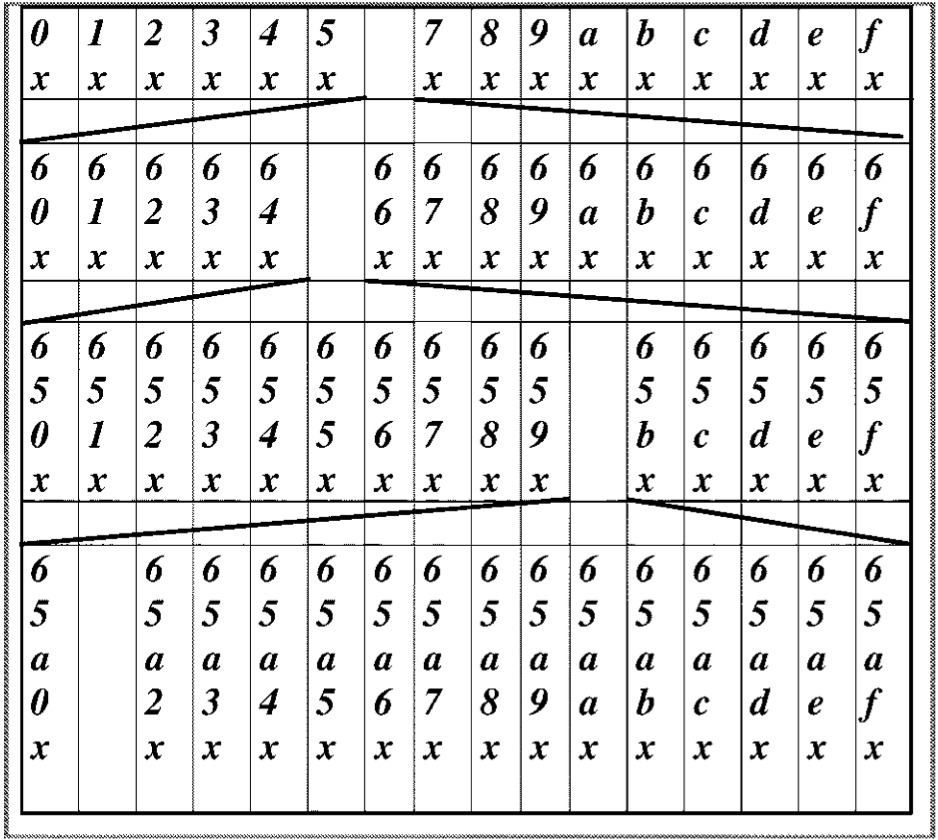
\includegraphics[scale=0.19]{img/pastry_table.png}
    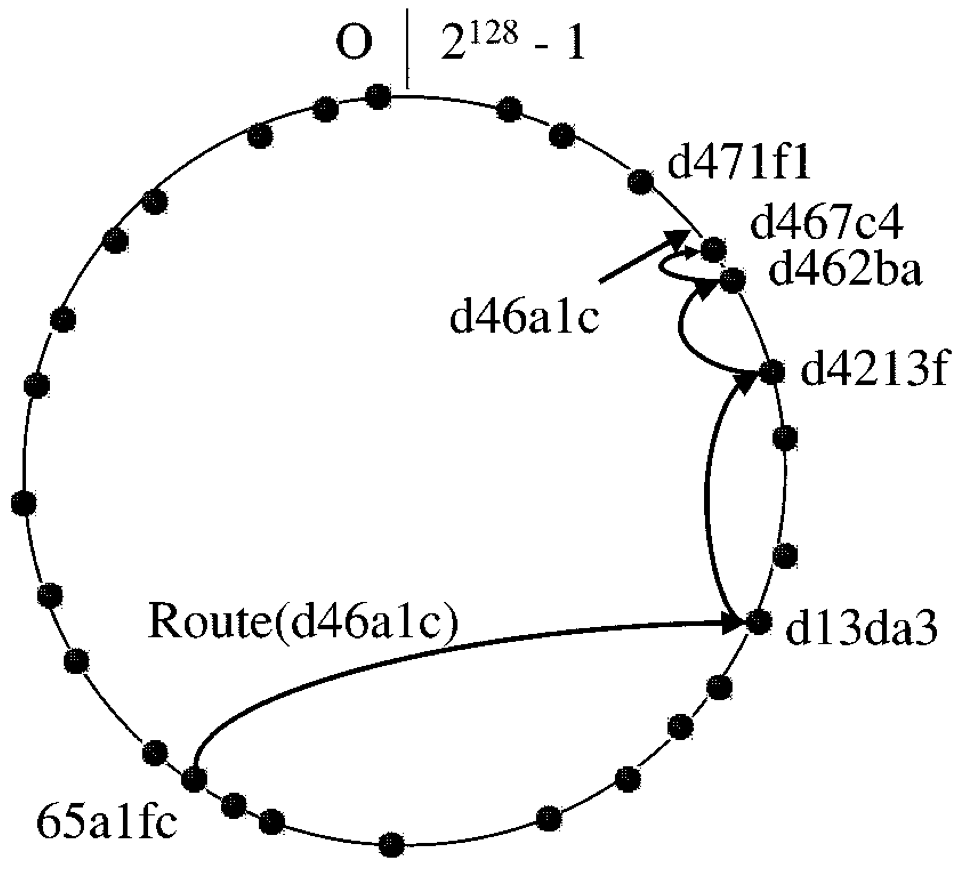
\includegraphics[scale=0.19]{img/pastry_routing.png}
    \caption{From
        left to right, the structure of a routing table in Pastry and an
        example of the Pastry routing scheme, where a message from node
        \emph{65a1fc} with key \emph{d46a1c} is delivered to the rendezvous
        node (figures borrowed from~\cite{Castro:2002})}
\end{figure*}

Scribe~\cite{Castro:2002} builds a dissemination overlay on top of
Pastry~\cite{Rowstron:2001}, a distributed hash table (DHT) which provides other
protocols with routing capabilities through an API\@. Scribe leverages
these capabilities in order to provide group and membership management
as well as message dissemination.

In Scribe, a tree structure is constructed for each group (i.e.\ topic).
When a node wants to publish a message, it sends the message to the root
node of the dissemination tree for the particular topic. This node is
referred to as a \emph{rendezvous node}, and is responsible for
disseminating the publication to its children. The initial phase of the
dissemination, where the message is routed to the rendezvous node, is
handled by Pastry. Pastry uses a routing scheme based on unique node ids
living in a circular namespace. Each node maintains a routing table of
such ids, where each row $n$ contains a sequence that match the id of
the current node in the $n$ first digits. When a node performs a lookup
in the routing table, it will traverse the table like a tree. It will
start by iterating through the entries in the first row until it finds a
id sequence which matches the key on the very first digit, then it will
lookup the row where the node ids all start with this digit, and iterate
through the entries until it finds the sequence which is a match on both
the first and the second digit. This will continue until an entry is
found which shares a prefix with the lookup key which is longer than the
current node id. If no such id is found, it will find an entry with
a prefix with the same size as the current node id, but where the following
digit is closer to the key. When the publication reaches the rendezvous
node, this node will continue the dissemination by forwarding the
publication to its children.

\section{The PeerNet Simulator}
PeerNet is an extended version of the
popular \emph{PeerSim simulator}~\cite{p2p09-peersim}. More
specifically, PeerNet adds a distributed simulation mode, where each
node, or a subset of nodes, can be executed in separate processes. This
means that unlike PeerSim, where execution of the protocols are
performed sequentially, each node in PeerNet is able to execute
concurrently. Also, in contrast with PeerSim, the execution of the
system happens in real-time. The higher degree of parallelism and
the real-time execution are two important factors which enable PeerNet to
provide a more realistic environment for running experiments. It is also
worth to mention that running in distributed mode is beneficial with
regard to scalability in terms of number of nodes included in the
simulation, as the memory and computational resources required to run
the simulation can be distributed across several machines. This is an
important factor as PeerNet is implemented in Java, which is a fairly
memory intense language when dealing with large-scale systems.

While PeerNet is able to extend PeerSim with a distributed mode, it also
provides a simulation mode which behaves exactly like simulations in
PeerSim, where experiments are run locally in one single process. In our
evaluation, we take advantage of both simulation modes in PeerNet. We
update existing PeerSim implementations of PolderCast and Scribe for use
with PeerNet, as well as implement a \emph{reporter interface} for these
protocols in order to make them compatible with our tool for visualizing
and evaluating such systems.
